\subsection{U-Net}\label{s:unet}
\chapterauthor{Woon Jun Wei (2200624)}

The U-Net architecture, introduced by Ronneberger et al. in 2015, is a pioneering model for biomedical image segmentation, widely adopted for various image segmentation tasks \cite{ronneberger_u-net_2015}. U-Net features a symmetric architecture with a contracting path to capture context and an expansive path for precise localization. The architecture includes skip connections that concatenate feature maps from the contracting path to the expanding path, enhancing the segmentation performance (see Figure \ref{f:unet}).

\begin{figure}[H] 
	\centering
	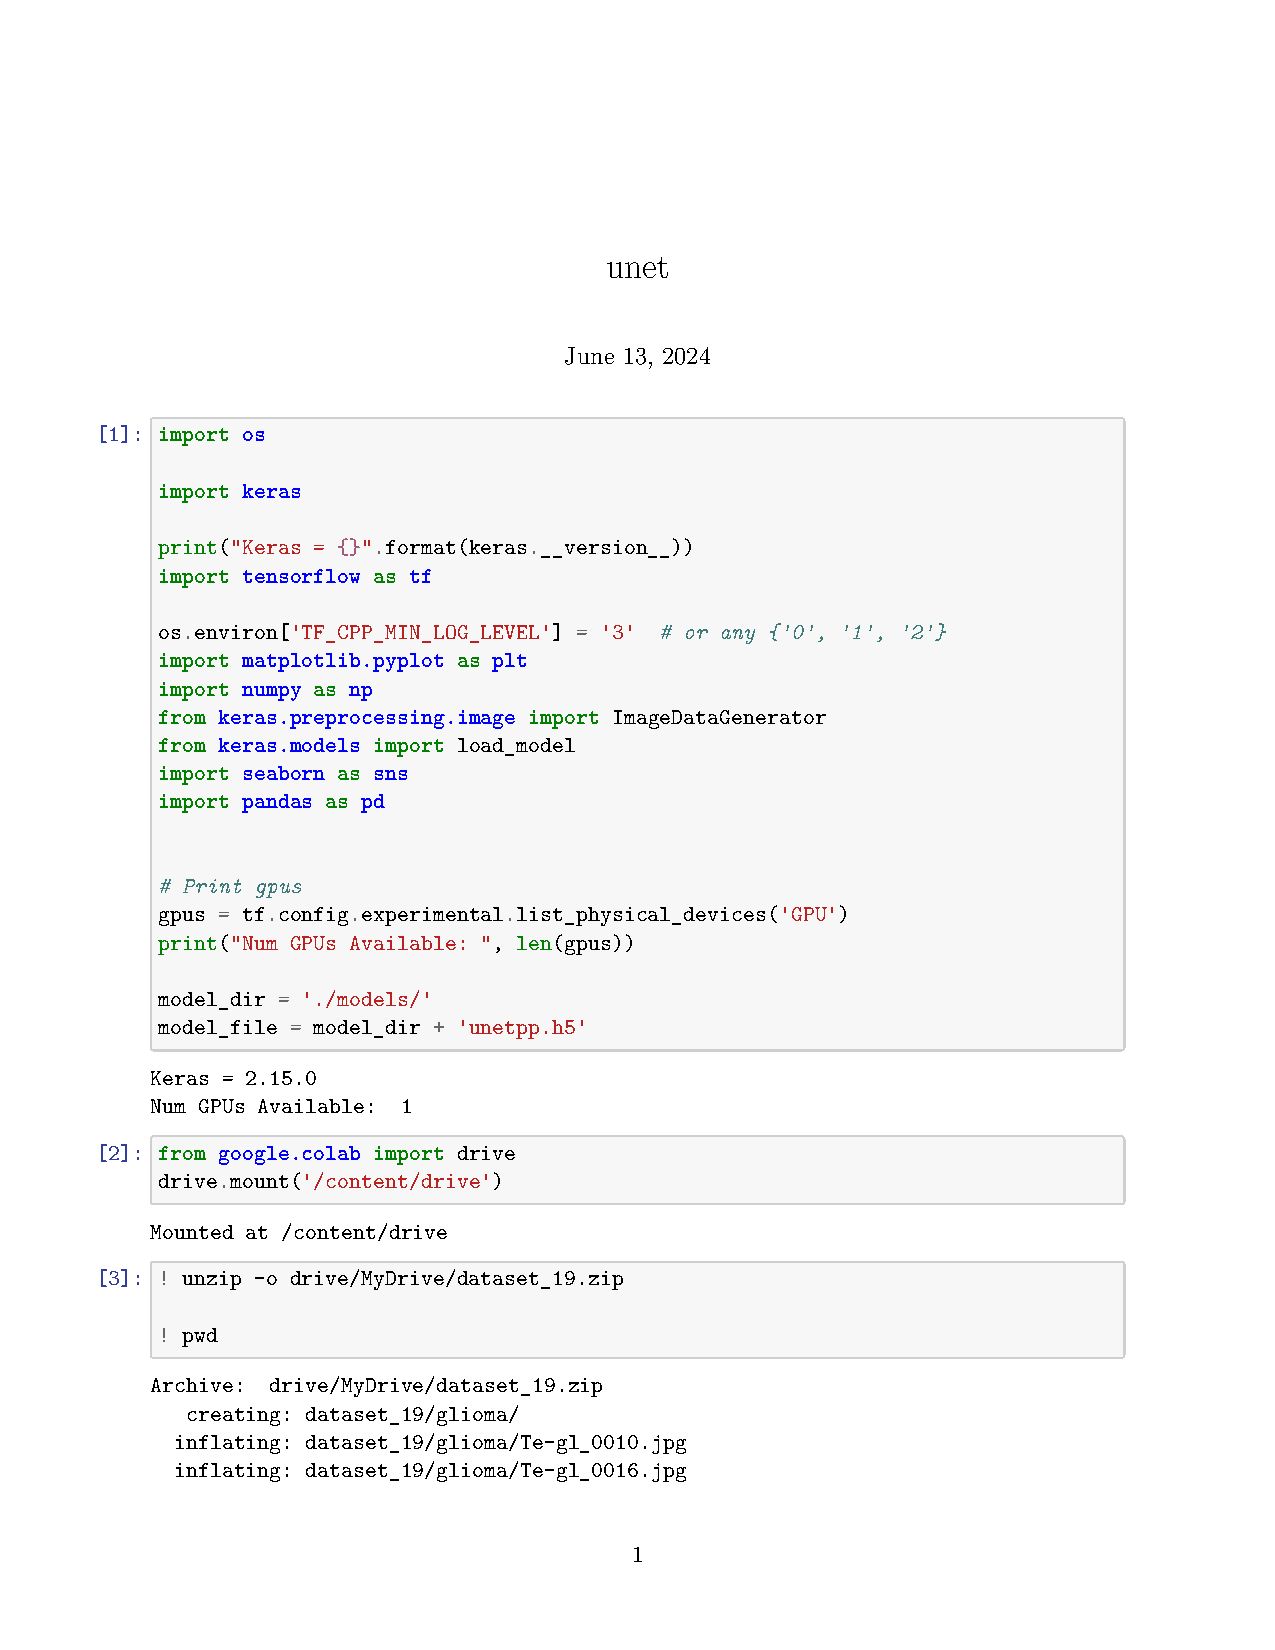
\includegraphics[width=0.5\textwidth]{unet/unet.png}
	\caption{Simple U-Net architecture}\label{f:unet}
\end{figure}

\subsubsection{Implementation}

U-Net++, an extension introduced by Zhou et al. in 2018, improves the original architecture by incorporating dense skip connections. These connections concatenate feature maps from all previous layers in the contracting path to the expanding path, enhancing feature reuse and segmentation accuracy \cite{zhou_unet_2018}.

Due to the complexity and time constraints associated with training, evaluation, and tuning, a U-Net model was not architected from scratch. Instead, this study employed the U-Net++ architecture using the \texttt{segmentation\_models} library. This library offers implementations of various deep learning models for image segmentation, supporting pre-trained models such as VGG, ResNet, and EfficientNet as down-sampling backbones.

Input images were preprocessed by cropping, enhancing, and resizing to $244 \times 244 \times 3$, as detailed in Section \ref{image_cropping_enhancement}. Further preprocessing included normalization, horizontal flipping, and random rotation by 20 degrees, managed by the \texttt{ImageDataGenerator} class, which also handled the 80:20 training-validation split.

The implemented model architecture was U-Net++ with an EfficientNetB0 backbone, initialized with ImageNet weights. To obtain classification results for the full image instead of pixel-wise classification, a Global Average Pooling layer followed by a Dense layer with four units and a softmax activation function was added. The model was compiled using the categorical cross-entropy loss function and accuracy metric.

Training was conducted using the Adam optimizer with a learning rate of 0.0001 and a batch size of 10 for 100 epochs. The best model was saved based on validation loss, incorporating Checkpointing, Early Stopping, and Reduce Learning Rate on Plateau. Training halted at 23 epochs due to early stopping, achieving a validation loss of 0.05597 and a validation accuracy of 0.9778.

\subsubsection{Results and Evaluation}

\begin{figure}[H]
  \begin{center}
    \includegraphics[width=0.35\textwidth]{unet/evaluation/cm1.png}
    \includegraphics[width=0.35\textwidth]{unet/evaluation/cm2.png}
    \includegraphics[width=0.35\textwidth]{unet/evaluation/ROC.png}
    \includegraphics[width=0.35\textwidth]{unet/evaluation/learning_curve.png}
  \end{center}
  \caption{Confusion Matrix, ROC Curve, and Learning Curve for Brain Tumor Segmentation}\label{f:unet_evaluation}
\end{figure}


\begin{longtable}{|l|c|c|c|c|}
\caption{Classification Report for Brain Tumor Segmentation} \label{tab:unet_classification_report}
\hline \textbf{Class} & \textbf{Precision} & \textbf{Recall} & \textbf{F1-Score} & \textbf{Support} \\ \hline 
\endfirsthead

\multicolumn{5}{c}%
{{\bfseries \tablename\ \thetable{} -- continued from previous page}} \\
\hline \textbf{Class} & \textbf{Precision} & \textbf{Recall} & \textbf{F1-Score} & \textbf{Support} \\ \hline 
\endhead

\hline \multicolumn{5}{|r|}{{Continued on next page}} \\ \hline
\endfoot

\hline
\endlastfoot

meningioma & 1.00 & 0.96 & 0.98 & 24 \\ \hline
pituitary  & 0.96 & 0.96 & 0.96 & 24 \\ \hline
glioma     & 0.96 & 1.00 & 0.98 & 24 \\ \hline
notumor    & 1.00 & 1.00 & 1.00 & 24 \\ \hline
micro avg  & 0.98 & 0.98 & 0.98 & 96 \\ \hline
macro avg  & 0.98 & 0.98 & 0.98 & 96 \\ \hline
weighted avg & 0.98 & 0.98 & 0.98 & 96 \\ \hline
samples avg & 0.98 & 0.98 & 0.98 & 96 \\ 
\end{longtable}

\begin{longtable}{|c|c|c|c|}
\caption{Additional Metrics for Brain Tumor Segmentation} \label{tab:unet_additional_metrics}
\hline \textbf{DSC} & \textbf{Sensitivity} & \textbf{Specificity} & \textbf{Accuracy} \\ \hline
\endfirsthead

\multicolumn{4}{c}%
{{\bfseries \tablename\ \thetable{} -- continued from previous page}} \\
\hline \textbf{DSC} & \textbf{Sensitivity} & \textbf{Specificity} & \textbf{Accuracy} \\ \hline
\endhead

\hline \multicolumn{4}{|r|}{{Continued on next page}} \\ \hline
\endfoot

\hline
\endlastfoot

% DSC: 0.9791621435808366, Sensitivity: 0.9791666666666667, Specificity: 0.9930555555555556, Accuracy: 0.9791666666666666
0.9792 & 0.9792 & 0.9931 & 0.9792 \\
\end{longtable}

% TBC
